\documentclass[pdftex,english,oribibl]{llncs}

%% Spracheinstellungen laden
\usepackage[english]{babel}

%% Schriftart in der Ausgabe/Eingabe
\usepackage[T1]{fontenc}
\usepackage{textcomp}
\usepackage[latin1]{inputenc}

%% Zitate
\usepackage[numbers]{natbib}
\bibliographystyle{abbrvnat}
\bibliographystyle{abnt-num}
%\bibliographystyle{dinat}
%\bibliographystyle{plainnat}
%\bibliographystyle{splncs}
%% Similar to option "sectionbib" but \refname instead of \bibname
\makeatletter
\renewcommand\bibsection{\section*{\refname\@mkboth{\MakeUppercase{\refname}}{\MakeUppercase{\refname}}}}
\makeatother

%% Index
%\usepackage{makeidx}
%\makeindex

%% PDF Einstellungen
% muss nach natbib geladen werden!
\usepackage{nameref}
\usepackage{varioref}
\usepackage[pdfusetitle,pdftex,colorlinks]{hyperref}
\hypersetup{pdfborder={0 0 0}}
\hypersetup{bookmarksdepth=3}
\hypersetup{bookmarksopen=true}
\hypersetup{bookmarksopenlevel=1}
\hypersetup{bookmarksnumbered=true}
\usepackage{color}
\hypersetup{colorlinks=false}

%\usepackage[section]{tocbibind}

\makeatletter
\gdef\@keywords{}
\def\keywords#1{\gdef\@keywords{#1}}
\gdef\@subtitle{}
\def\subtitle#1{\gdef\@subtitle{#1}}

%% modified from llncs
\renewenvironment{abstract}{%
  \list{}{\advance\topsep by0.35cm\relax\small%
          \leftmargin=1cm%
          \labelwidth=\z@%
          \listparindent=\z@%
          \itemindent\listparindent%
          \rightmargin\leftmargin}%
          \item[\hskip\labelsep\bfseries\abstractname]}{%
  \if!\@keywords!\else{\item[~]\item[\hskip\labelsep\bfseries\keywordname]\@keywords}\fi%
  \endlist}

\AtBeginDocument{%
  \if!\@subtitle!\else\hypersetup{pdfsubject={\@subtitle}}\fi
  \if!\@keywords!\else\hypersetup{pdfkeywords={\@keywords}}\fi
}
\makeatother

% llncs hyperref fix
\makeatletter
\providecommand*{\toclevel@author}{0}
\providecommand*{\toclevel@title}{0}
\makeatother

%% Grafiken
\usepackage[pdftex]{graphicx}
\DeclareGraphicsExtensions{.pdf,.jpg,.png}
\usepackage{subfigure}

%% Mathe
\usepackage{amsmath}
\usepackage{amssymb}

%% Listings
\usepackage{listings}
\lstset{escapechar=\%, frame=tb, basicstyle=\footnotesize}

%% Sonstiges
\newcommand{\TODO}[1]{\par\textcolor{red}{#1}\marginpar{\textcolor{red}{TODO}}}
\newcommand{\TODOX}[1]{\textcolor{red}{#1}\marginpar{\textcolor{red}{TODO}}}
\pagestyle{plain}

% Keine "Schusterjungen"
\clubpenalty = 10000
% Keine "Hurenkinder"
\widowpenalty = 10000 \displaywidowpenalty = 10000

%%%%%%%%%%%%%%%%%%%%%%%%%%%%%%%%%%%%%%%%%%%%%%%%%%%%%%%%%%%%%%%%%%%%%%%%%%%%%%%
%%% BEGIN DOCUMENT
%%%%%%%%%%%%%%%%%%%%%%%%%%%%%%%%%%%%%%%%%%%%%%%%%%%%%%%%%%%%%%%%%%%%%%%%%%%%%%%
\title{Security Evaluation}
% \subtitle{My (optional) Subtitle}
\author{Prince Thomas}
\institute{University of Stuttgart\\Institute of Software Technology (ISTE)\\70569 Stuttgart, Germany}


\begin{document}

\maketitle

\begin{abstract}
Software security is an idea implemented to secure software against malicious attack and other hacker risks so that the software continues to function correctly under such potential risks. Security is necessary to provide integrity, authentication and availability. The fast growth rate of software and software products makes the software security aspect even more critical. Most organizations these days want their information system to be managed as safely as possible. Security Evaluation is the basic step in achieving this goal for any organization. Security Evaluation is particularly important because of the rapidly changing environment of the information security system or the operation system.In this survey we are performing a study on Software Security Evaluation techniques. A detailed analysis of Qualitative and Quantitative Security Evaluation approaches is being carried out. The suitability and challenges of different methods of each of this approach is studied. The systems where these techniques are being used are investigated to understand the performance of security evaluation methods. Finally, the paper is concluded with the scope of the different security evaluation approaches for real time systems.
\end{abstract}

\section{Introduction}

  Software security is the idea of engineering software so that it continues to function correctly under malicious attack \cite{1281254} .The fast-growing software systems and huge amount of data handling makes the software security an important aspect in Modern software development. Software security has to be evaluated to make sure that software is minimally susceptible to threats. Evaluation of software security is so challenging because of the non-predictability of the threats and attacker behaviors.

  Introduce the different sections of this paper shortly in one or two sentences.

  
\section{Importance of Security Evaluation}
Why do we need Security Evaluation?

\section{Software Security Metrics}
Metrics is a measurement standard which defines what is to be measured, how to be measured and helps the security practitioners to manage the product efficiently. Security metrics is the powerful tool that helps security practitioners to integrate security features into their system. The security metrics are gaining lot of significance now a days because with the help of the data obtained from them software security decisions can be taken and which in turn helps the software developers to secure their software product. 

Security metrics help in decision making regarding security-related attributes of a process, system, or organization. In particular, security metrics can be applied to compare the effectiveness of different security mechanisms, or to indicate the degree to which security requirements of an organization are being met. In addition, they can also be used to systematically improve the security level of a system, or to predict this security level in a future point in time. All the people involved in the software life cycle from developers to users use the security metrics for different use cases. For example Technical Personnels(Developers) use security metrics to decide which configuration change is the most effective to increase network resilience, Management members for financial investment on security and finally end users for the trustworthiness of a software products available in the market.

The desired properties of a good security metric are granularity, availability, cost effectiveness, localization and validation\cite{8017389}. 

\subsection{Importance of Software Security Metrics}
Significance of security Metrics
\subsection{Classification of Security Metrics}
The security metrics can be classified as fig\ref{fig:security_metric_types} \cite{8017389}.

\begin{figure}
	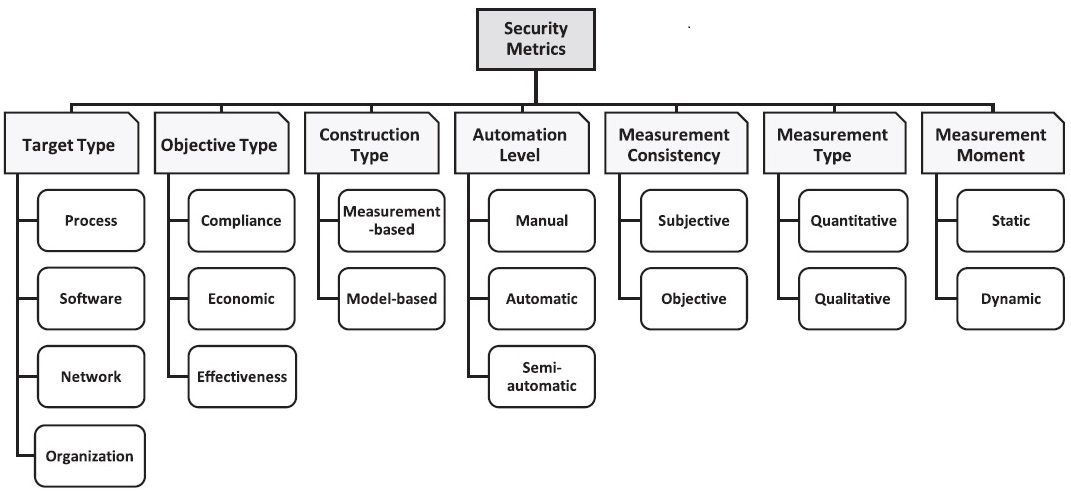
\includegraphics[width=\linewidth]{figures/security_metric_types.jpg}
	\caption{Classification of Security Metrics}
	\label{fig:security_metric_types}
\end{figure}

\begin{enumerate}
	\item {\textbf{Target Type:} Security metrics can be categorized according to the target they evaluate. The most common targets assessed (and respective security metrics) are the following:}
	\begin{enumerate}
		\item {\textbf{Process:} Process security metrics quantify the security level of a product by assessing its associated development process.}
		\item {\textbf{Software:} Software security metrics evaluate software security by assessing source code defects, software (mis)configuration, or other vulnerabilities present in software components.}
		\item {\textbf{Network:} Network Security Metrics(NSMs) assess the security of entire networks or parts thereof.}
		\item {\textbf{Organization:} Organization security metrics evaluate the physical and personnel security of an organization.}
	\end{enumerate}

	\item {\textbf{Objective Type:} Based on its objective type security metric can be classified as:}
	\begin{enumerate}
	\item {\textbf{Compliance:} Compliance security metrics measures how well the security requirements of a target is being met based on the security methods and policies.}
	\item {\textbf{Economic:} Metrics taking into consideration of the financial aspects of security.}
	\item {\textbf{Effectiveness:} It measures how effectively the security measures can perform against security threats or violations.}
	\end{enumerate}

	\item {\textbf{Construction Type:} Based on the way security metrics is derived, they can be classified as:}
	\begin{enumerate}
	\item {\textbf{Measurement-based:} This security metric is used to quantify the security property that is being measured.}
	\item {\textbf{Model-based:} Here the metrics values are derived from the complex mathematical equations used to define the formal mathematical model of the target. Refer fig\ref{fig:modelbased_metric} for a simple representation of a model-based security metric. Examples of models used to evaluate security metrics are attack graphs, Markov models, attack trees, Bayesian networks, etc. In the following sections the detailed evaluation of model-based security metrics is described.}

	\begin{figure}
		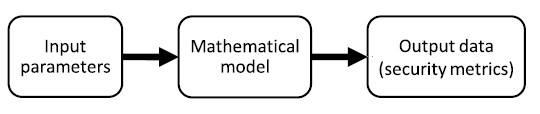
\includegraphics[width=\linewidth]{figures/modelbased_metric.jpg}
		\caption{Evaluation Process of Model-Based Security Metrics}
		\label{fig:modelbased_metric}
	\end{figure}
	\end{enumerate}

	\item {\textbf{Automation Level:} Based on the level of automation used for the measurements the security metric can be classified as:}
	\begin{enumerate}
	\item {\textbf{Manual:} The collection of metrics values are being carried out manually(by humans).}
	\item {\textbf{Automatic:} Metrics values are being collected with the help of computer system without the intervention of humans.}
	\item {\textbf{Semi-Automatic:} Measurement is carried out with the help of both humans and computer systems.}
	\end{enumerate}

	\item {\textbf{Measurement Consistency:} Corresponding to the consistency of the metric values, security metrics can be classified as:}
	\begin{enumerate}
	\item {\textbf{Subjective:} Security metric is subjective to the person performing the metric measurement. Different people evaluating the same security property using same method can produce different results.}
	\item {\textbf{Objective:} Same result is being obtained irrespective of the person performing the evaluation.}
	\end{enumerate}

	\item {\textbf{Measurement Type:} According to the type of the measurement security metrics can be classified as:}
	\begin{enumerate}
		\item {\textbf{Quantitative:} Quantitative security metrics are expressed as percentages or cardinal numbers (i.e., numbers that count something, instead of ordinal numbers, which only denote the position occupied by a given object).}
		\item {\textbf{Qualitative:} Qualitative security metrics are expressed by labels such as high-medium-low values. Ordinal numbers can also be regarded as qualitative values.}
	\end{enumerate}

	\item {\textbf{Measurement Moment:} Depending on the instance of time at which the security metrics are applied to assess a given target, they can be classified as either static or dynamic::}
	\begin{enumerate}
	\item {\textbf{Static:} Static, or pre-deployment, security metrics are developed to be measured before the assessed target enters operation.}
	\item {\textbf{Dynamic:} Dynamic, or run-time, security metrics are those developed to be constantly measured, during the operation of the target being evaluated.}
	\end{enumerate}

\end{enumerate}

Overview of different  Security Metrics\newline

	Security Metrics for Software Systems\cite{Wang:2009:SMS:1566445.1566509}\newline
	"Citation is missing" the paper name: Security Metrics for Software Systems\newline
	Phase Wise Review of Software Security Metrics\cite{Ansar:PWRSSM}\newline
	Survey on Systems Security Metrics\cite{Pendleton:2016:SSS:3022634.3005714}\newline
	
\section{Qualitative Software Security Evaluation Methods}
Different qualitative evaluation methods will be explained here.\newline
A short introduction about the qualitative approaches.\newline
Different subsections for different methods.\newline
Challenges of Qualitative Security Evaluation.\newline

	Qualitative analyzis of software security patterns\cite{5564015}\newline
 	Scenario based Security Evaluation\cite{Halkidis:2006:QAS:2639528.2639723}\newline
  	Vulnerability-centric and qualitative risk analysis method\cite{6165757}\newline
  	Software System with Vulnerability Life Cycle and User Profiles\cite{6532147}\newline
  	"Citation is missing" the paper name: Security Evaluation for Software System with Vulnerability Life Cycle and User Profiles\newline
  
\section{Quantitative Software Security Evaluation Methods}
Different quantitative evaluation methods will be explained here.\newline
A short introduction about the quantitative approaches.\newline
Different subsections for different methods.\newline
Challenges of Quantitative Security Evaluation.\newline

  	Quantifying the security attribute of an intrusion tolerant system\cite{1028941}\newline
  	Quantitative Security Evaluation for Software System from Vulnerability Database\cite{Okamura:2013:QSESVD}\newline
 	Model Based Evaluation, Stochastic approaches\cite{1335467}\newline
  	Quantitative evaluation:the vulnerability life cycle; and the attacker behaviour\cite{5315969}\newline
  	Machine learning and CVE data base to predict the vulnerabilities in the software\cite{Jain:2017:CAE:3102980.3102991}\newline
  	
\section{Case Study}
Different Real time examples where these security evaluation techniques are being used.\newline

	\cite{Kotenko}\newline
	"Citation is missing" the paper name: Attack Modelling and Security Evaluation in SIEM Systems\newline
	
\section{Conclusions}\label{sec:conclusions}
Mention the importance of the security evaluation again and scope of the same in real time scenarios.
Future scope of security evaluation methods.

\bibliography{template}

\end{document}
